%\CHComment{With the newly added section on exemplary case, perhaps we could re-organize this section? A couple of suggestions: 1) very briefly summarize the three cases and highlight the success stories in the introduction section; 2) move the detailed description of Table Migration and Service Fabric into the experience section.}

\subsection{Azure Storage vNext}
\label{sec:cases:azurestore}

%Azure Storage vNext is the next generation storage system for Windows Azure. Azure Storage vNext consists of multiple extent managers, extent nodes, and network engines that are able to send messages across the network, and enqueue any received messages in the input queue of the corresponding node (see Figure~\ref{fig:azurestore}). Each extent manager is responsible for managing a subset of the extent nodes. Each extent node stores its corresponding extent in a local storage, and sends periodical heartbeats and synchronization messages to the extent manager. When the extent manager receives a synchronization message it is responsible to update extent nodes with the latest extent.

%\begin{figure}[t]
%\centering
%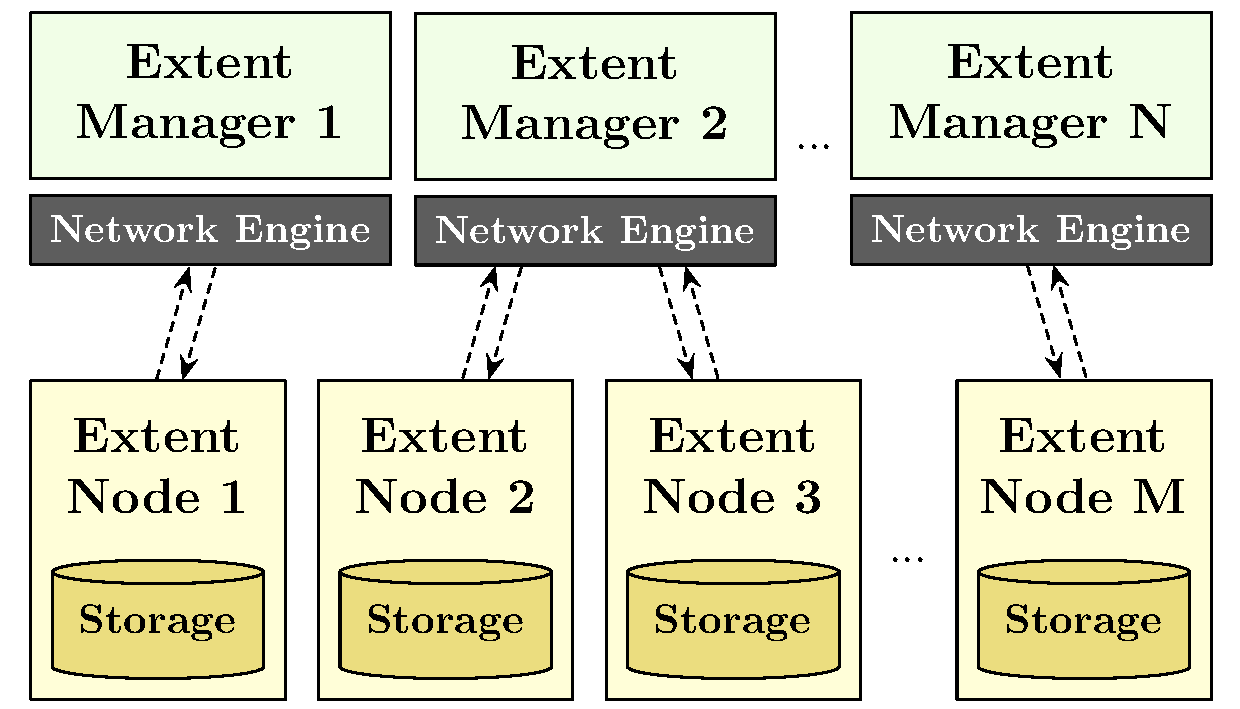
\includegraphics[width=\linewidth]{img/azurestore}
%\caption{Top-level components of a distributed extent management system for Windows Azure.}
%\label{fig:azurestore}
%\end{figure}

%The liveness property that must be always eventually satisfied in the Azure Storage vNext system is that a user-defined $N$ number of extent nodes must be always eventually available with the latest extent. There was an actual bug in the system, that led this property to fail for some very rare executions. Although this buggy behavior would be observed from time to time during stress testing, there was no way to reproduce the bug. We discuss later in this paper, how we are able to detect and reproduce this bug using our approach.

%Azure Storage vNext is very challenging to test. All the unit test and integration test suites of the Azure Storage vNext project successfully pass every single time. However, the developers found that the stress test suite, which constantly kills and launches extent nodes, could fail from time to time after very long executions. The observed failure was that the liveness property described in Section~\ref{sec:overview:bugs} would not get satisfied. The developers had no way to deterministically reproduce this bug or be able to detect what is the culprit, as the traces they were getting were very long and hard to parse.

vNext bug goes here.

\subsection{Live Azure Table Migration}
\label{sec:cases:migration}

The Live Azure Table Migration is a library capable of transparently migrating a data set between tables in the Windows Azure storage service while an application is accessing the data set.  MigratingTable provides a \emph{virtual table} with an API similar to that of an ordinary Azure table, backed by a pair of \emph{old} and \emph{new}  tables.  A background \emph{migrator} job moves all data from the old table to the new table.  Meanwhile, each read or write issued to the virtual table is translated to a sequence of reads and writes on the backend tables according to a protocol we designed, which guarantees linearizability of operations on the virtual table across multiple application processes assuming that the backend tables respect their own linearizability guarantees.

\begin{figure}[t]
\centering
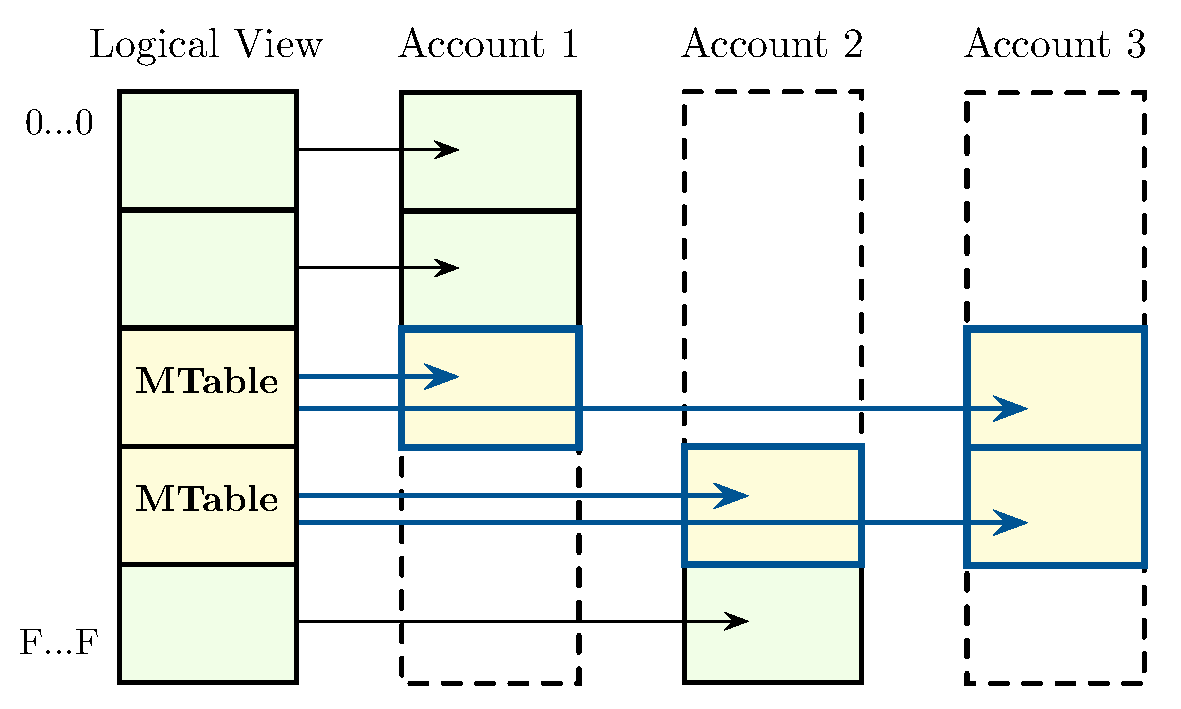
\includegraphics[width=\linewidth]{img/livemigration}
\caption{Resharding a data set when a third Azure storage account is added. Two key ranges are each migrated to the new account using a MigratingTable instance (abbreviated MTable).}
\label{fig:livemigration}
\end{figure}

% N.B. Artifact Services is mentioned at http://research.microsoft.com/en-us/people/schulte/.  Hopefully it's OK to reveal that it was the system in this case study. ~ Matt 2015-08-17
The initial motivation for MigratingTable was to solve a scaling problem for Artifact Services, an internal Microsoft system with a data set that is sharded across tables in different Azure storage accounts because it exceeds the limit on traffic supported by a single Azure storage account.  As the traffic continues to grow over time, the system needs to reshard the data set across a greater number of Azure storage accounts without interrupting service.  During such a resharding, our sharding manager will identify each key range that should migrate to a different table, and we will use a separate MigratingTable instance for each such key range to actually perform the migration (Figure~\ref{fig:livemigration}).  MigratingTable may also be useful to migrate data to a table with different values of configuration parameters that Azure does not support changing on an existing table, such as geographic location.

\subsection{Azure Service Fabric (change to CScale?)}
\label{sec:cases:fabric}

\PDComment{I guess we should write stuff about CScale here based on our last discussion: overview of the system (collection of Fabric services connected via TPL dataflow?), of its environment (Fabric), how they interop?, why its very challenging to test? how they test currently? I am not sure if all these should go here or be split here and the experience report, we will see ... same for the above case studies}

\emph{Azure Service Faric} (or \emph{Fabric} for short)
is a platform and API for creating reliable services
that execute on a cluster of machines.
The developer writes a service that receives requests (e.g.\ from some client program via HTTP)
and mutates its state based on these requests.
In order to make the service \emph{reliable},
Fabric launches several copies (\emph{replicas}) of the service,
where each copy runs as a separate process
on different nodes in the cluster.
One replica is selected to be the \emph{primary}
which serves client requests; the rest are \emph{secondaries}.
The primary replicates state changes to the secondaries
so that all replicas eventually have the same state.
If the primary fails (e.g.\ if the node on which the primary is running crashes),
Fabric elects one of the secondaries to be the new primary
and launches another secondary;
the new secondary will receive a full or partial copy (depending on whether persistent storage is used) 
of the state of the new primary in order to ``catch up'' with the other secondaries. 
Fabric provides a name-resolution service so that clients can always find the current primary.
Fabric exposes several different APIs that developers can use to write services.































